\documentclass[12pt,a4paper]{report}  %紙張設定
\usepackage{xeCJK}%中文字體模組
%\setCJKmainfont{標楷體} %設定中文字體
\setCJKmainfont{MoeStandardKai.ttf}
%\newfontfamily\sectionef{Times New Roman}%設定英文字體
\newfontfamily\sectionef{Nimbus Roman}
\usepackage{enumerate}
\usepackage{amsmath,amssymb}%數學公式、符號
\usepackage{amsfonts} %數學簍空的英文字
\usepackage{graphicx, subfigure}%圖形
\usepackage{fontawesome5} %引用icon
\usepackage{type1cm} %調整字體絕對大小
\usepackage{textpos} %設定文字絕對位置
\usepackage[top=2.5truecm,bottom=2.5truecm,
left=3truecm,right=2.5truecm]{geometry}
\usepackage{titlesec} %目錄標題設定模組
\usepackage{titletoc} %目錄內容設定模組
\usepackage{textcomp} %表格設定模組
\usepackage{multirow} %合併行
%\usepackage{multicol} %合併欄
\usepackage{CJK} %中文模組
\usepackage{CJKnumb} %中文數字模組
\usepackage{wallpaper} %浮水印
\usepackage{listings} %引用程式碼
\usepackage{hyperref} %引用url連結
\usepackage{setspace}
\usepackage{lscape}%設定橫式
\lstset{language=Python, %設定語言
		basicstyle=\fontsize{10pt}{2pt}\selectfont, %設定程式內文字體大小
		frame=lines,	%設定程式框架為線
}
%\usepackage{subcaption}%副圖標
\graphicspath{{./../images/}} %圖片預設讀取路徑
\usepackage{indentfirst} %設定開頭縮排模組
\renewcommand{\figurename}{\Large 圖.} %更改圖片標題名稱
\renewcommand{\tablename}{\Large 表.}
\renewcommand{\lstlistingname}{\Large 程式.} %設定程式標示名稱
\hoffset=-5mm %調整左右邊界
\voffset=-8mm %調整上下邊界
\setlength{\parindent}{3em}%設定首行行距縮排
\usepackage{appendix} %附錄
\usepackage{diagbox}%引用表格
\usepackage{multirow}%表格置中
%\usepackage{number line}
%=------------------更改標題內容----------------------=%
\titleformat{\chapter}[hang]{\center\sectionef\fontsize{20pt}{1pt}\bfseries}{\LARGE 第\CJKnumber{\thechapter}章}{1em}{}[]
\titleformat{\section}[hang]{\sectionef\fontsize{18pt}{2.5pt}\bfseries}{{\thesection}}{0.5em}{}[]
\titleformat{\subsection}[hang]{\sectionef\fontsize{18pt}{2.5pt}\bfseries}{{\thesubsection}}{1em}{}[]
%=------------------更改目錄內容-----------------------=%
\titlecontents{chapter}[11mm]{}{\sectionef\fontsize{18pt}{2.5pt}\bfseries\makebox[3.5em][l]
{第\CJKnumber{\thecontentslabel}章}}{}{\titlerule*[0.7pc]{.}\contentspage}
\titlecontents{section}[18mm]{}{\sectionef\LARGE\makebox[1.5em][l]
{\thecontentslabel}}{}{\titlerule*[0.7pc]{.}\contentspage}
\titlecontents{subsection}[4em]{}{\sectionef\Large\makebox[2.5em][l]{{\thecontentslabel}}}{}{\titlerule*[0.7pc]{.}\contentspage}
%=----------------------章節間距----------------------=%
\titlespacing*{\chapter} {0pt}{0pt}{18pt}
\titlespacing*{\section} {0pt}{12pt}{6pt}
\titlespacing*{\subsection} {0pt}{6pt}{6pt}
%=----------------------標題-------------------------=%             
\begin{document} %文件
\sectionef %設定英文字體啟用
\vspace{12em}
\begin{titlepage}%開頭
\begin{center}   %標題  
\makebox[1.5\width][s] %[s] 代表 Stretch the interword space in text across the entire width
{\fontsize{24pt}{2.5pt}國立虎尾科技大學}\\[18pt]
\makebox[1.5\width][s]
{\fontsize{24pt}{2.5pt}機械設計工程系}\\[18pt]
\sectionef\fontsize{24pt}{1em}\selectfont\textbf
{
\vspace{0.5em}
cd2023 2a-pj1ag4分組報告}\\[18pt]
%設定文字盒子 [方框寬度的1.5倍寬][對其方式為文字平均分分布於方框中]\\距離下方18pt
\vspace{1em} %下移
\fontsize{30pt}{1pt}\selectfont\textbf{網際手足球機器人場景設計}\\
\vspace{1em}
\sectionef\fontsize{30pt}{1em}\selectfont\textbf
{
\vspace{0.5em}
Web-based Robot Soccer Scene Design}
 \vspace{1em}
%=---------------------參與人員-----------------------=%             
\end{center}
\begin{flushleft}
\begin{LARGE}

\hspace{32mm}\makebox[5cm][s]
{指導教授:\quad 嚴\quad 家\quad 銘\quad 老\quad 師}\\[6pt]
\hspace{32mm}\makebox[5cm][s]
{班\qquad 級:\quad 四\quad 設\quad 二\quad 甲}\\[6pt]
\hspace{32mm}\makebox[5cm][s]
{學\qquad 生:\quad 洪\quad 偉\quad 陞\quad(41023146)}
\\[6pt]
\hspace{32mm}\makebox[5cm][s]
{\hspace{43mm}夏\quad 進\quad 源\quad(41023148)}\\[6pt]
\hspace{32mm}\makebox[5cm][s]
{\hspace{43mm}紀\quad  閔\quad 翔\quad(41023147)}\\[6pt]
\hspace{32mm}\makebox[5cm][s]
{\hspace{43mm}施\quad 建\quad 昌\quad(41023143)}\\[6pt]
\hspace{32mm}\makebox[5cm][s]
{\hspace{43mm}李\quad 承\quad 翰\quad(41023121)}\\[6pt]
\hspace{32mm}\makebox[5cm][s]
{\hspace{43mm}林\quad 建\quad 維\quad(41023134)}\\[6pt]
\hspace{32mm}\makebox[5cm][s]
{\hspace{43mm}呂\quad 佳\quad 柔\quad(41023104)}\\[6pt]
\hspace{32mm}\makebox[5cm][s]
{\hspace{43mm}王\quad 啟\quad 騰\quad(41023112)}\\[6pt]
%設定文字盒子[寬度為5cm][對其方式為文字平均分分布於方框中]空白距離{36.5mm}\空白1em
\end{LARGE}
\end{flushleft}
\vspace{4em}
\fontsize{18pt}{2pt}\selectfont\centerline{\makebox[\width][s]
{中華民國\hspace{3em} 
112 \quad 年\quad 6\quad 月}}
\end{titlepage}
\newpage


%=------------------------摘要-----------------------=%
\renewcommand{\baselinestretch}{1.5} %設定行距
\pagenumbering{roman} %設定頁數為羅馬數字
\clearpage  %設定頁數開始編譯
\sectionef
\addcontentsline{toc}{chapter}{摘~~~要} %將摘要加入目錄
\begin{center}
\LARGE\textbf{摘~~要}\\
\end{center}
\begin{flushleft}
\fontsize{14pt}{20pt}\sectionef\hspace{12pt}\quad 本學期採取個人及團體分組來學習,團體實習目標為開發一款能在 web-based CoppeliaSim 場景中雙方或多方對玩的遊戲。pj3 為八人一組,根據自選產品在期限內完成產品開發,在 w16 現場發表八人協同四週後所完成的產品,在 w17 各組採 OBS + Teams 以影片發表所完成的協同產品。\\[12pt]
\fontsize{14pt}{20pt}\sectionef\hspace{12pt}\quad  接續 pj2,各組須對雙輪車進行設計改良,以提升行進與對戰效率。採 CAD 進行場景與多輪車零組件設計後,轉入足球場景中以鍵盤 arrow keys 與 wasd 等按鍵進行控制,對雙方每組將有四名輪車球員,且每兩人在同一台電腦上操作,完成後各組須在分組網站中提供所有相關檔案下載連結,且提供線上分組簡報與分組 pdf 報告連結。\\[12pt]	
\fontsize{14pt}{20pt}\sectionef\hspace{12pt}\quad 此專題是雙方利用各四台 BubbleRob 多輪車在一足球場景中進行對戰,雙方球門分別設有感測器。 在規定時間內,每進一球即透過程式重新往球場內隨機發球,接續賽局。模擬場景中還須配置 LED 計分板顯示比賽剩餘時間與比分,還需另外建立以機械轉盤傳動計分系統。在 CoppeliaSim 模擬環境中進行測試運用上的可行性並嘗試透過埠號供使用者觀看。\\
  更多詳細內容可以到 https://mdecd2023.github.io/2a3-pj3ag4 了解。\\[10pt]

\end{flushleft}
\newpage
%=--------------------Abstract----------------------=%
\renewcommand{\baselinestretch}{1.5} %設定行距
\addcontentsline{toc}{chapter}{Abstract} %將摘要加入目錄
\begin{center}
\LARGE\textbf\sectionef{Abstract}\\
\begin{flushleft}
\fontsize{14pt}{16pt}\sectionef\hspace{12pt}\quad This semester adopts both individual and group learning approaches. The group project involves developing a web-based game that allows two or more players to interact in a CoppeliaSim simulation environment. For Project 3 (pj3), the group consists of eight members who will collaborate to develop a product of their choice within a given deadline. In Week 16, the group will present the product they have developed over four weeks of collaboration. In Week 17, each group will use OBS + Teams to present their collaborative product through a video presentation.\\[12pt]
\fontsize{14pt}{16pt}\sectionef\hspace{12pt}\quad Continuing from pj2, each group is required to design improvements for a two-wheeled vehicle to enhance its mobility and combat efficiency. Using CAD software, the groups will design the scene and components of the multi-wheel vehicle. The project will then transition to a soccer field scenario, where the vehicle will be controlled using keyboard arrow keys and WASD keys. Each group will have four vehicle players, with two players operating on the same computer. Upon completion, each group must provide download links for all relevant files on the group's website, as well as links to online group presentations and a PDF report.\\[12pt]
\fontsize{14pt}{16pt}\sectionef\hspace{12pt}\quad This project involves a two-player battle using four BubbleRob multi-wheel vehicles in a soccer field scenario. Each player has their own goal equipped with sensors. Within a specified time frame, each goal scored triggers the program to reset and randomly kick off a new ball into the field, continuing the game. The simulation scene also includes an LED scoreboard to display the remaining time and score of the match. Additionally, a mechanical turntable-driven scoring system needs to be created. Feasibility testing and user observation will be conducted in the CoppeliaSim simulation environment, with the option for users to observe through port numbers.\\[12pt]
\end{flushleft}

\newpage
%=------------------------目錄----------------------=%
\renewcommand{\contentsname}{\centerline{\fontsize{18pt}{\baselineskip}\selectfont\textbf{目\quad 錄}}}
\tableofcontents  %目錄產生
\newpage
%=------------------圖表目錄產生----------------------=%
\renewcommand{\listfigurename}{\centerline{\fontsize{18pt}{\baselineskip}\selectfont\textbf{圖\quad 目\quad 錄 }}}
\newcommand{\loflabel}{圖} %定義\loflabel 文字為圖
\renewcommand{\numberline}[1]{\loflabel~#1\hspace*{0.5em}}
\listoffigures
%\newcommand{\captioname}{圖}
%\newpage
%\renewcommand{\listtablename}{\centerline{\fontsize{18pt}{\baselineskip}\selectfont\textbf{表\quad 目\quad 錄 }}}
%\newcommand{\lotlabel}{表} %定義\lotlabel 文字為表
%\renewcommand{\numberline}[1]{\lotlabel~#1\hspace*{0.5em}}
%\listoftables

\end{center}
%=-------------------------內容----------------------=%
\chapter{前言}
\renewcommand{\baselinestretch}{10.0} %設定行距
\pagenumbering{arabic} %設定頁號阿拉伯數字
\setcounter{page}{1}  %設定頁數
\fontsize{14pt}{2.5pt}\sectionef
\section{設計架構}
此次 pj3 專題目標有建立場景中的計時器、球員外型及移動優化、添加球員擊球和翻車再起能、進球後收集並隨機投下新的一顆球、建立以機械式轉盤傳動計分系統。由於目標繁多,需要組員間分工負責,在每個禮拜的協同中逐步完成 pj3 專題。\\

\begin{figure}[hbt!]
\begin{center}
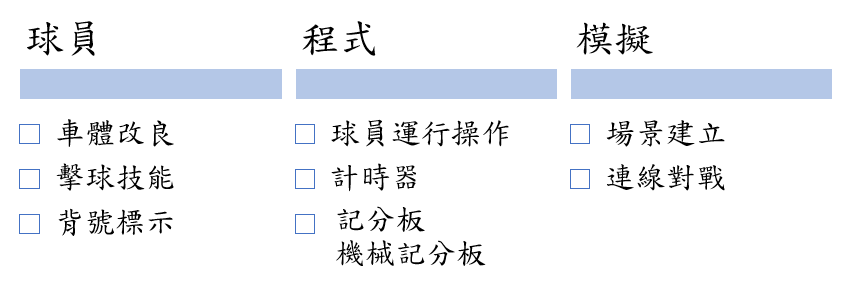
\includegraphics[width=15cm]{35}
\caption{\Large 設計目標圖}\label{fig.35}
\end{center}
\end{figure}
\section{規則說明}\emph{}
類似於足球遊戲,一開始時球會置於場中央,遊戲開始後雙方即可以鍵盤操控機器人,透過防守敵方以及與隊友間的傳球推球至已方的球門得分。\\
遊戲規則如下:
\begin{enumerate}
\item 球觸碰到球門感測器即算得分。
\item 在十分鐘的比賽時間內,獲得最多分數的隊伍即獲勝。
\item 任一方進球得分後,隨機在場內投下新的球,雙方接續進行比賽。
\end{enumerate}

\renewcommand{\baselinestretch}{0.5} %設定行距
\chapter{球員製作過程}
\renewcommand{\baselinestretch}{10.0} %設定行距
\pagenumbering{arabic} %設定頁號阿拉伯數字
\setcounter{page}{2}  %設定頁數
\fontsize{14pt}{2.5pt}\sectionef
\section{車體改良-運行}
  原本的車體為球形 BubbleRob,雖然造型簡單,卻會有容易翻車的問題。因此改為磚塊型,在前後添加兩顆輪子保持平衡。也將前進原理改為四輪驅動,使轉彎更為順暢合理。\\[1pt]
\begin{figure}[hbt!]
\begin{center}
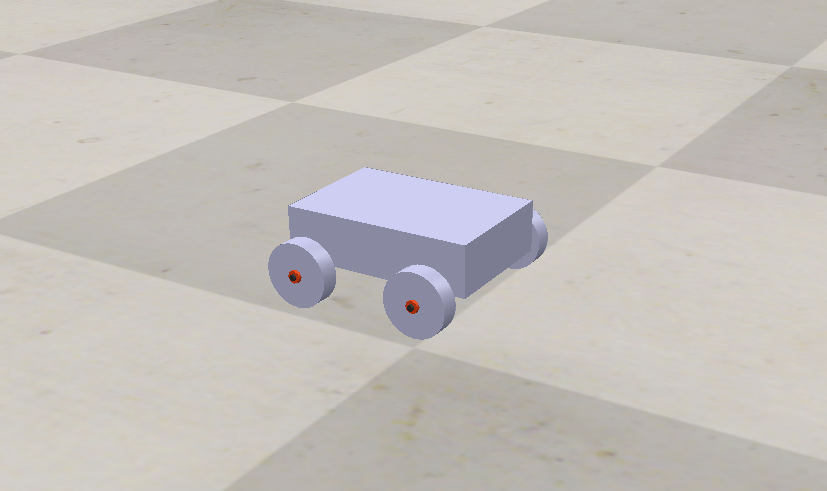
\includegraphics[height=5cm]{36}
\caption{\Large 磚塊型車體}\label{fig.36}
\end{center}
\end{figure} 
\section{車體改良-擊球}
  球員前端添加凸出的手部,球員本體在 CoppeliaSim 中用導入的開啟方式會產生抖動,因此改為加入物件 skin 並將本體隱藏。\\
\begin{figure}[hbt!]
\begin{center}
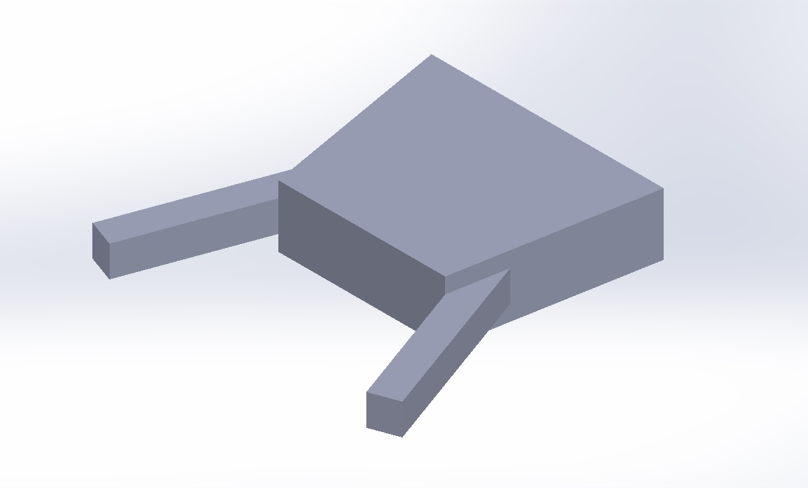
\includegraphics[height=4cm]{37}
\caption{\Large 球員 skin}\label{fig.37}
\end{center}
\end{figure} 
\newpage
\section{車體改良-背號}
  由於兩隊各有四名球員,場上總共八名球員,為了能更清楚觀看及辨別球員,除了透過顏色區分隊伍,也需要讓每個球員添加背號。第一版的背號是直立式置於球員上方,實際遊玩時發現會有影響重心的問題。\\
\begin{figure}[hbt!]
\begin{center}
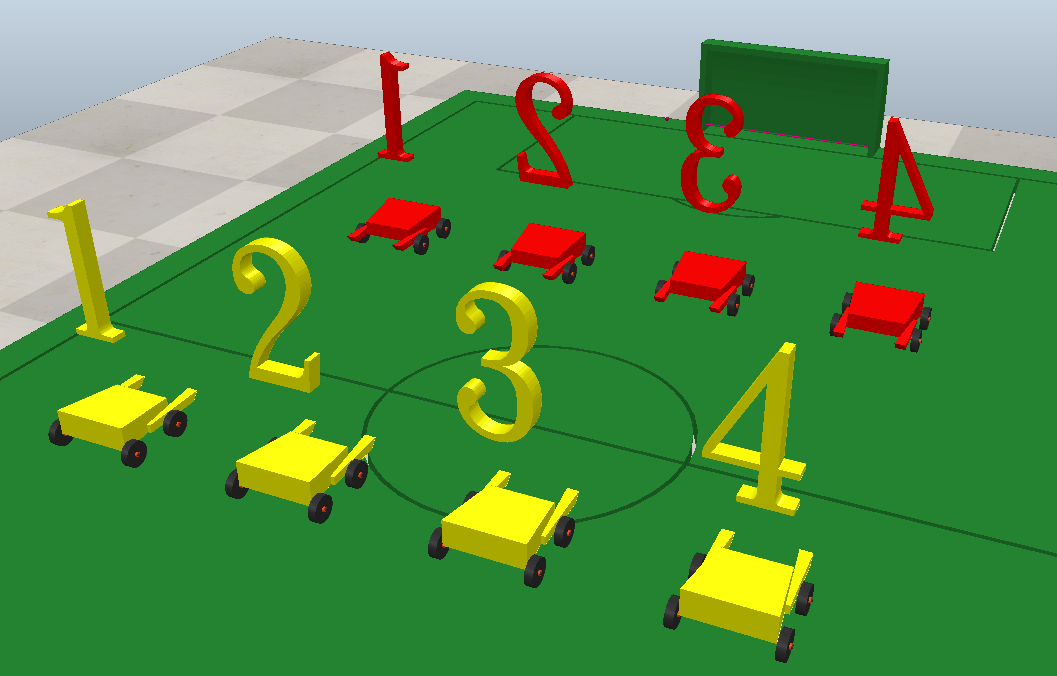
\includegraphics[height=6cm]{38}
\caption{\Large 第一版球員背號}\label{fig.38}
\end{center}
\end{figure}


於是第二版做了調整,參考實際賽車都將編號繪於車身,我們將背號改為平貼於車頂,解決了影響重心的問題。\\
\begin{figure}[hbt!]
\begin{center}
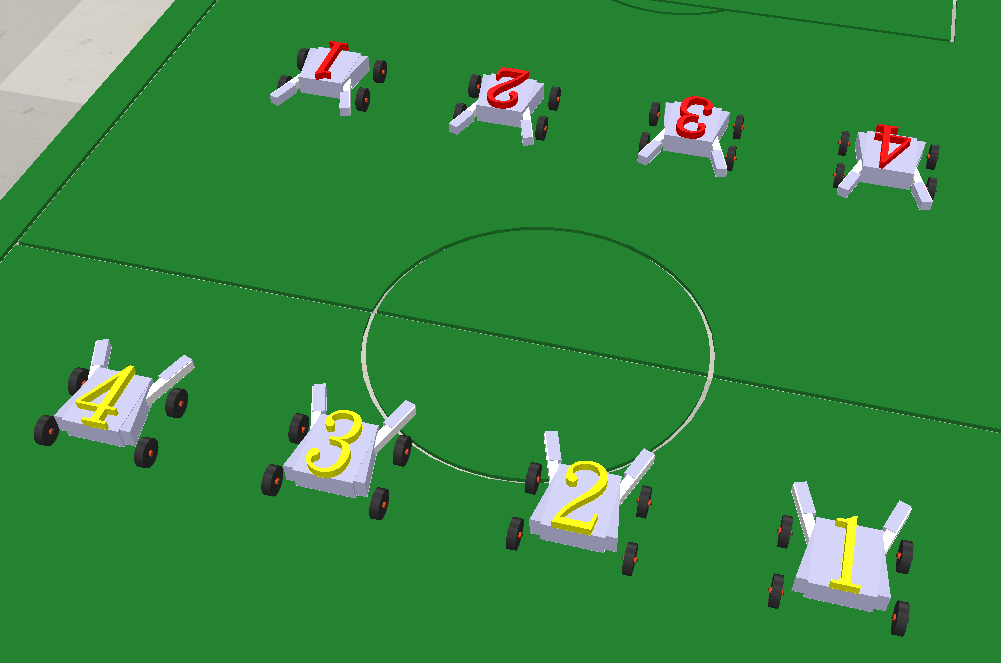
\includegraphics[height=6cm]{39}
\caption{\Large 第二版球員背號}\label{fig.39}
\end{center}
\end{figure}

\renewcommand{\baselinestretch}{1} %設定行距
\chapter{球員程式碼}
\renewcommand{\baselinestretch}{10.0} %設定行距
\pagenumbering{arabic} %設定頁號阿拉伯數字
\setcounter{page}{4}  %設定頁數
\fontsize{14pt}{2.5pt}\sectionef
\section{車體改良-操作}
  為了增加對戰的刺激性及操作的方便性,我們對球員的程式碼新增可以前後移動並同時左右移動還有添加倒地翻身的功能。\\[1pt]

\section{移動操作-輪子旋轉}
\begin{figure}[hbt!]
\begin{center},
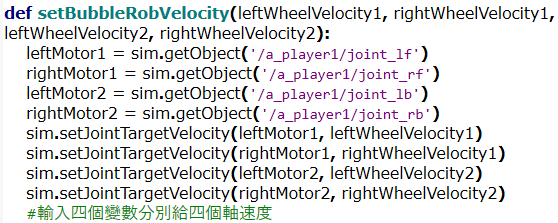
\includegraphics[height=6cm]{40}
\caption{\Large 設定球員輪子旋轉}\label{fig.40}
\end{center}
\end{figure}
(圖.\ref{fig.40}) 設定一個 setVelocity 函數,接受四個參數:leftWheelVelocity1,rightWheelVelocity1,leftWheelVelocity2,rightWheelVelocity2,分別為左右前後輪速度。在函數內部使用 sim.getObject() 函數獲取左右前後輪的關節 joint ,並使用 sim.setJointTargetVelocity() 函數將各關節的目標速度設置為傳入的參數值,這樣做及可控制球員輪子速度,從而使球員移動。\\
\newpage
\section{移動操作-前輪方向}
\begin{figure}[hbt!]
\begin{center}
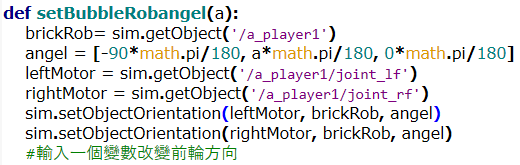
\includegraphics[height=4cm]{41}
\caption{\Large 設定球員前輪方向}\label{fig.41}
\end{center}
\end{figure}
(圖.\ref{fig.41}) 設定一個 setBubbleRobange1 函數,接受一個設置角度值得參數 "a",以函數 sim.getObject 獲取一個代表 "a player"模型的對象"brickRob"。計算角度值並傳入參數"a"轉換為弧度值,將另兩個角度分別為固定角度值。在使用 sim.getObject() 獲取左右前輪的關節,以 sim.setObjectOrientation() 將關節地朝向設置為與 brickRob 相對應的角度,便可以給定角度旋轉並改變球員地朝向位置。\\
\section{移動操作-左右轉向}
\begin{figure}[hbt!]
\begin{center}
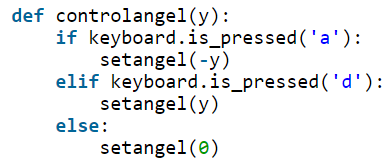
\includegraphics[height=4cm]{42}
\caption{\Large 控制球員左右轉向}\label{fig.42}
\end{center}
\end{figure}
(圖.\ref{fig.42}) controlange1 函數接受控制角度的函數"y",檢查按鍵輸入,按下"a"調用 setangel(-y) ,將傳入函數取相反值設成角度;按下"d"則用 setangel(y),傳入函數直接設成角度;無按下任何鍵則調用 setangel(0),將角度設為零。\\
  此程式碼根據按鍵輸入來控制角度值輸入,可以分別控制向左向右角度值。\\
\section{移動操作-控制球員移動}
\begin{figure}[hbt!]
\begin{center}
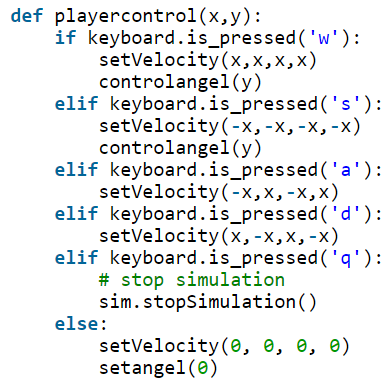
\includegraphics[height=8cm]{43}
\caption{\Large wasd移動球員}\label{fig.43}
\end{center}
\end{figure}
(圖.\ref{fig.43}) 以 playcontrol 函數定義參數"x"和"y",代表速度及角度。檢查按鍵輸入,如果按下"w"將調用 setVelocity(x, x, x, x)設置輪子速度、調用 controlangel(y) 控制角度。若為 setVelocity(-x, -x, -x, -x)則設置為反向速度,按下"q"則停止模擬。\\
  根據鍵盤輸入 w, a, s, d 來控制球員前進、後退、左轉和右轉。\\
\newpage
\section{移動操作-維持速度}
\begin{figure}[hbt!]
\begin{center}
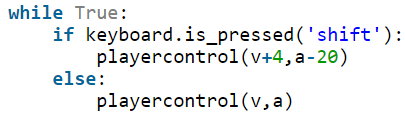
\includegraphics[height=3cm]{44}
\caption{\Large 控制球員速度}\label{fig.44}
\end{center}
\end{figure}
(圖.\ref{fig.44}) 此程式碼使用無限循環"while True"迴圈,如果按下"shift"會調用 playcontrol(v+4, a-20)函數,使原有速度增加4,角度減去20。使用無線循環迴圈檢測鍵盤輸入,調整速度與角度。\\
\section{球員改良-倒地翻身}
\begin{figure}[hbt!]
\begin{center}
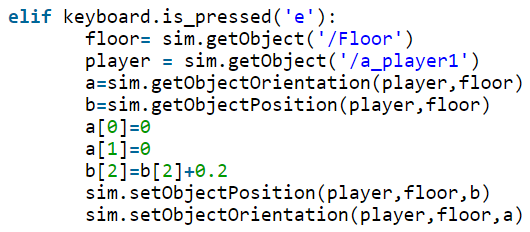
\includegraphics[height=5cm]{45}
\caption{\Large 控制球員翻身}\label{fig.45}
\end{center}
\end{figure}
(圖.\ref{fig.45}) 定義如果按"e"就執行,以 sim.getObject('/Floor') 獲取地板句柄、('/a player1') 球員句柄;sim.getObjectOrientation(player,floor) 獲取相對於地板的球員方向、Position(player,floor) 獲取相對於地板的球員位置,將數值存於變量"a"及"b"中。a[0]=0 將球員的x角度為0,a[1]=0 將球員的y角度為0,b[2]=b[2]+0.2 將球員的z位置上升0.2。最後通過 sim.setObjectPosition(player,floor,b) 設定球員相對於地板的位置、Orientation(player,floor,a) 設定球員相對於地板的方向。\\
  此段程式碼根據按下"e"來執行將指定對象地朝向與位置進行修改,使球員翻倒後能夠再次翻身站起,繼續進行比賽。\\
\renewcommand{\baselinestretch}{1} %設定行距
\chapter{計時器與記分板}
\renewcommand{\baselinestretch}{10.0} %設定行距
\pagenumbering{arabic} %設定頁號阿拉伯數字
\setcounter{page}{8}  %設定頁數
\fontsize{14pt}{2.5pt}\sectionef
\section{摘要}
  完成球員設定後,接著說明場景中計時器設定與 LED 記分板和機械式轉盤記分板製作過程。\\
\section{計時器}
\begin{figure}[hbt!]
\begin{center}
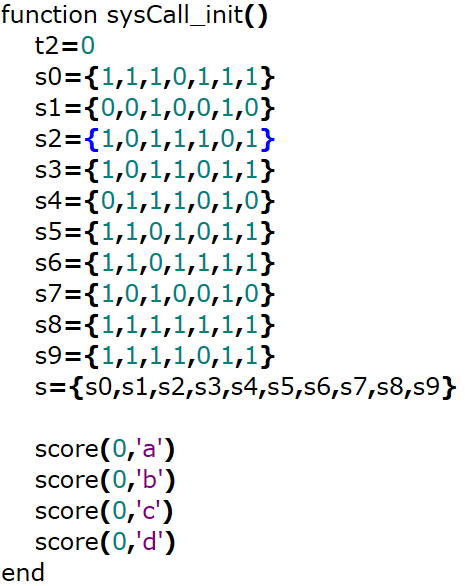
\includegraphics[height=8cm]{46}
\caption{\Large 定義變量}\label{fig.46}
\end{center}
\end{figure}
(圖.\ref{46}) 以函數 sysCall init 定義一些變量,將 t2 初始化為 0,s0 到 s9 由 0 到 1 組成的列表,用於後續計算。通過調用 score(0, 'a')、score(0, 'b')、score(0, 'c')和 score(0, 'd') 來初始化名為 a、b、c、d 的得分。\\
  此程式碼做用是在模擬環境初始化階段定義一些變量、列表及得分的部分。\\
\newpage
\begin{figure}[hbt!]
\begin{center}
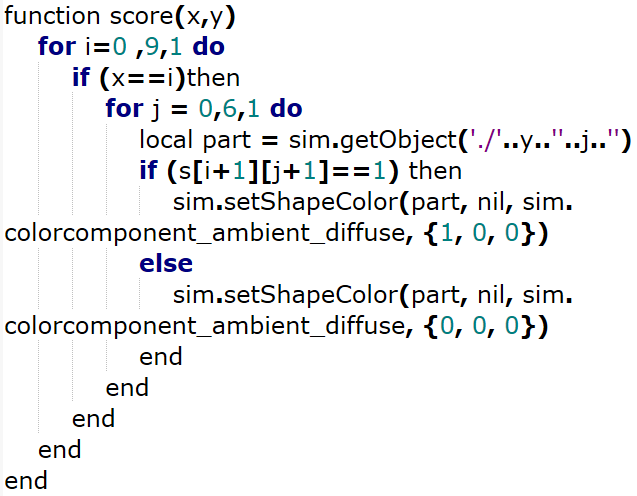
\includegraphics[height=8cm]{47}
\caption{\Large 數字顏色}\label{fig.47}
\end{center}
\end{figure}
(圖.\ref{47}) score 函數接受參數 "x"、"y",使用一個循環重複數字 0 到 9,首先檢查"x"是否等於當前數字,如果相等則執行內部循環。以 sim.getObject() 根據給定的字符串構建對象名稱並儲存在 part 變量中。再檢查 s[i+1][j+1] ,數字 i 在位置 j 上如果為 1 就使用 sim.setShapeColor() 將 part 對象的顏色設置為紅色 ({1, 0, 0}),若非則將顏色設置為黑色 ({0, 0, 0})。\\
  根據輸入的數字"x"、"y"設置對應數字的顏色,以數字的模式在模擬環境中的相對應位置設置不同的顏色。\\
\newpage
\begin{figure}[hbt!]
\begin{center}
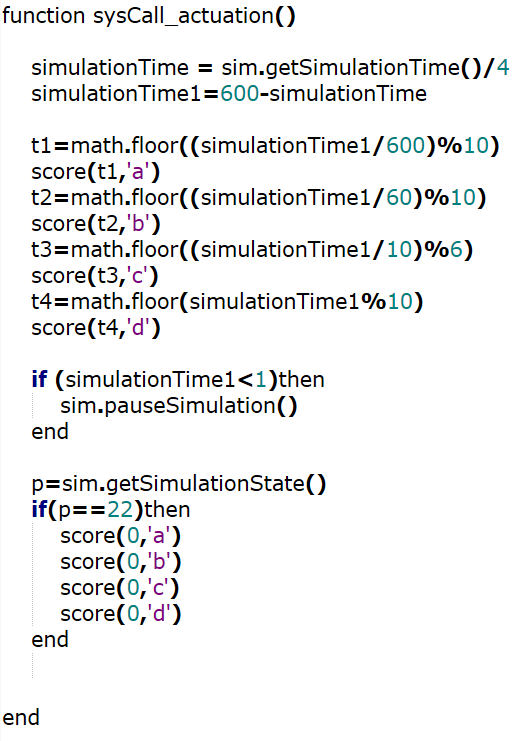
\includegraphics[height=9cm]{48}
\caption{\Large 更改數字形狀的顏色}\label{fig.48}
\end{center}
\end{figure}

(圖.\ref{48}) sysCall actuation 在模擬時被調用,首先藉由 sim.getSimulationTime() 獲取當前時間並除以4,儲存在變量 simulationTime 中。以 simulationTime 計算"t1"、"t2"、"t3"及"t4",分別表示當前時間的不同部分,所得值通過 simulationTime1 除以相對應數字,並取整數部分。\\
再來以 score() 將計算得到的值分別與"a"、"b"、"c"、"d"一起傳遞,可以根據時間的變化來更新相應的數字形狀的顏色。\\
  根據模擬時間的變化更新數字形狀的顏色,在特定條件下暫停模擬或重置顯示的顏色。\\
\begin{figure}[hbt!]
\begin{center}
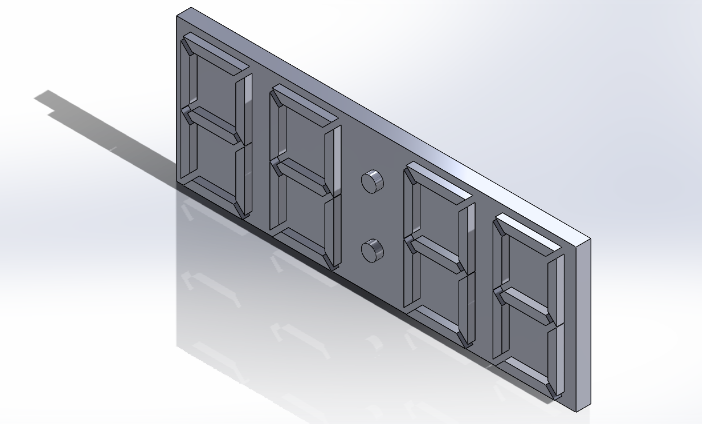
\includegraphics[width=6cm]{49}
\caption{\Large 計時器}\label{fig.49}
\end{center}
\end{figure}
\newpage
\section{LED記分板}
\begin{figure}[hbt!]
\begin{center}
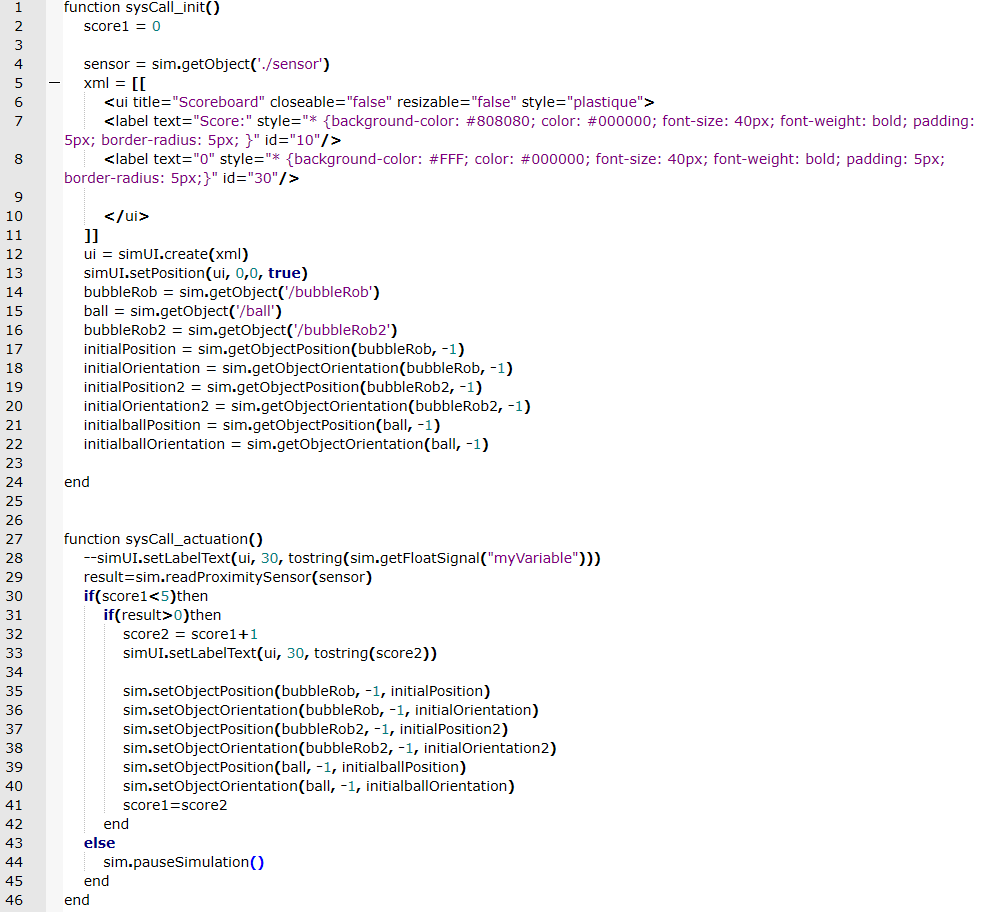
\includegraphics[width=16cm]{50}
\caption{\Large 記分板}\label{50}
\end{center}
\end{figure}
透過 Lua 程式建立記分板,設計樣式,給予偵測定義。\\
\newpage
\begin{figure}[hbt!]
\begin{center}
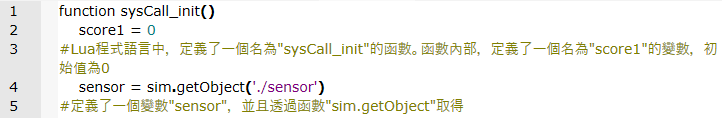
\includegraphics[width=16cm]{51}
\caption{\Large sensor}\label{51}
\end{center}
\end{figure}

(圖.\ref{51})sysCall init 的函式建立了一個名為 score1 的變數,並將它的值設定為 0使用 sim.getObject 方法來獲取一個名為 sensor 的物件,並將它儲存在 sensor 變數中。\\
\begin{figure}[hbt!]
\begin{center}
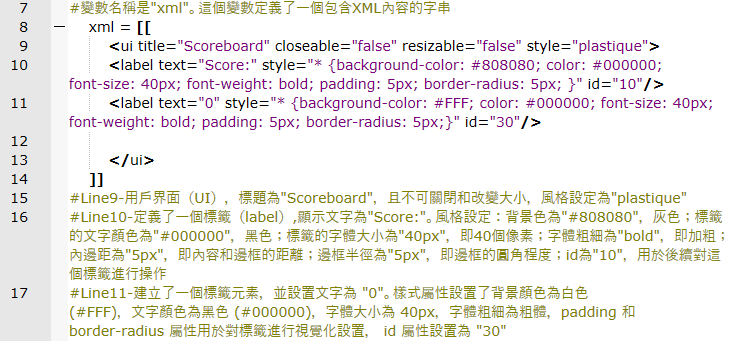
\includegraphics[width=16cm]{52}
\caption{\Large xml}\label{52}
\end{center}
\end{figure}

(圖.\ref{52}存儲在名為 xml 的變數中的 XML 代碼,它描述了一個顯示得分的視窗界面。ui 標籤中,有兩個 label 標籤,分別用來顯示 "Score:" 和得分。\\
\begin{figure}[hbt!]
\begin{center}
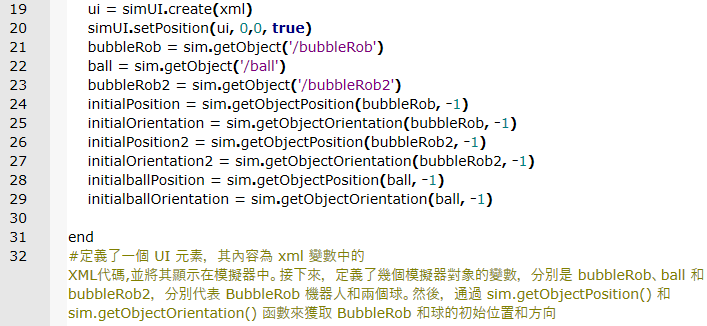
\includegraphics[width=16cm]{53}
\caption{\Large ui}\label{53}
\end{center}
\end{figure}

\newpage
(圖.\ref{53}建立使用者介面 (ui),然後設定該介面的位置為 (0, 0)。sim.getObject 函式從仿真場景中取得了三個物體,sim.getObjectPosition 和 sim.getObjectOrientation 函式取得了這些物體的初始位置和初始方向,這段程式碼是用來建立仿真場景中物體的初始位置和初始方向。\\
\begin{figure}[hbt!]
\begin{center}
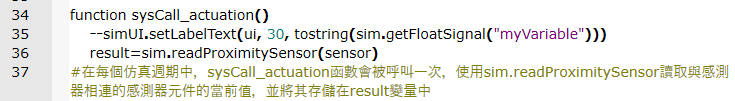
\includegraphics[width=16cm]{54}
\caption{\Large syscall}\label{54}
\end{center}
\end{figure}

(圖.\ref{54}sysCall-actuation的函式使用 sim.readProximitySensor 函式讀取一個接近傳感器的數據,並將結果儲存在 result 變數中。\\
\newpage
\begin{figure}[hbt!]
\begin{center}
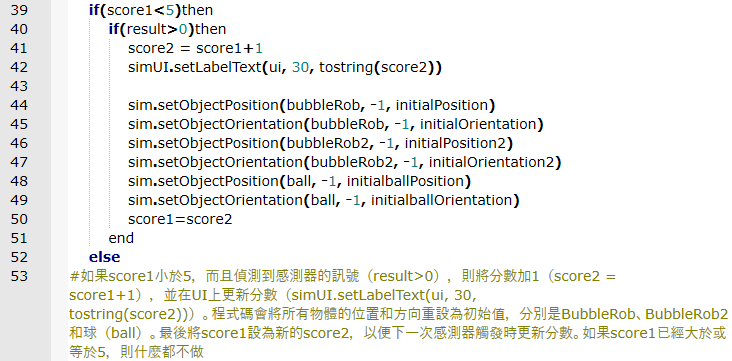
\includegraphics[width=16cm]{55}
\caption{\Large if-else}\label{55}
\end{center}
\end{figure}

(圖.\ref{55}這段程式碼的主要作用是檢查分數是否小於5分,如果 score1 的值小於5,且 result 大於0,則將分數加1並在ui上更新分數。如果 score1 的值已經達到或超過了5分,則會跳過。\\
\begin{figure}[hbt!]
\begin{center}
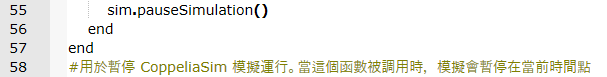
\includegraphics[width=16cm]{56}
\caption{\Large pause}\label{56}
\end{center}
\end{figure}

(圖.\ref{56}檢查分數是否小於5分。如果分數達到5分或更高,它會暫停仿真並結束程式執行。\\
\newpage
\section{機械式轉盤記分板}
  除了採用 LED 顯示計分外,另外建立以機械轉盤傳動計分系統,納入每按一下"i"轉盤及順時鐘旋轉36度。\\
\begin{figure}[hbt!]
\begin{center}
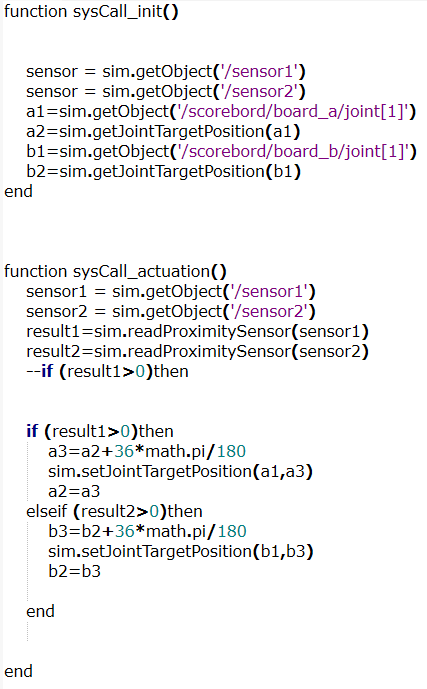
\includegraphics[width=9cm]{57}
\caption{\Large 機械記分板}\label{57}
\end{center}
\end{figure}
\newpage
\begin{figure}[hbt!]
\begin{center}
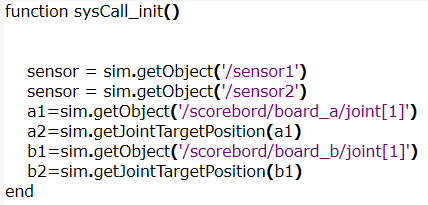
\includegraphics[width=8cm]{58}
\caption{\Large 獲取變量}\label{58}
\end{center}
\end{figure}
(圖.\ref{58} 使用 sim.getObject() 獲取 /sensor1 存入變量"sensor"、獲取 /scorebord/board a/joint[1] 的關節存入變量"a1",以 sim.getJointTargetPosition() 獲取"a1"目標位置存入變量"a2",獲取變量"b1"目標位置存入變量"b2"。\\
\begin{figure}[hbt!]
\begin{center}
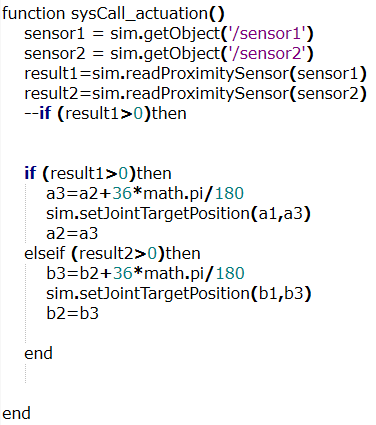
\includegraphics[width=6cm]{59}
\caption{\Large 角度偏移}\label{59}
\end{center}
\end{figure}

(圖.\ref{59} sim.readProximitySensor() 函數獲取近接傳感器 "sensor1"、"sensor2"的結果,存入變量"result1"、"result2",如果大於0則執行:關節"a1"的目標位置為當前位置"a2"加上36度的角度偏移,並將"a2"更新為"a3"以便下次執行使用。\\
  此程式碼根據接近傳感器的檢測結果來控制關節運動,使機械式轉盤隨比分計分。\\
\renewcommand{\baselinestretch}{0} %設定行距
\chapter{場景模擬}
\renewcommand{\baselinestretch}{10.0} %設定行距
\pagenumbering{arabic} %設定頁號阿拉伯數字
\setcounter{page}{17}  %設定頁數
\fontsize{14pt}{2.5pt}\sectionef
\section{摘要}
  完成球員及程式碼設定後,接著建立模擬場景,添加場地、球員、計時器、 LED 記分板和機械式轉盤記分板等等...。\\
\section{機械記分板放入場景}
  在 Coppeliasim 中導入 STL 圖檔,調整到合適方向,分別炸開物件,將數字部分調整成紅色,方便觀看。\\
\begin{figure}[hbt!]
\begin{center}
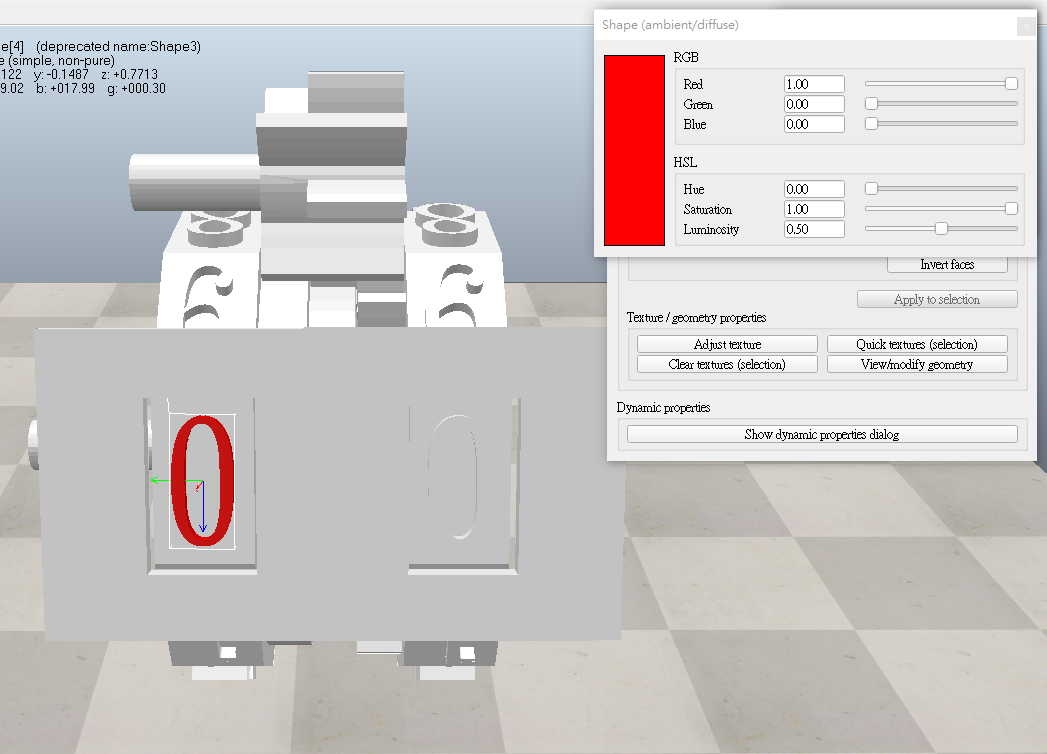
\includegraphics[height=6cm]{15}
\caption{\Large 數字調整顏色}\label{fig.15}
\end{center}
\end{figure}

  加入 joint 關節讓齒輪運轉,調整方位後依附在齒輪的中心軸上,除了主動軸外其他軸也要設定轉速為 0 ,避免模擬時齒輪隨意偏擺。\\
\begin{figure}[hbt!]
\begin{center}
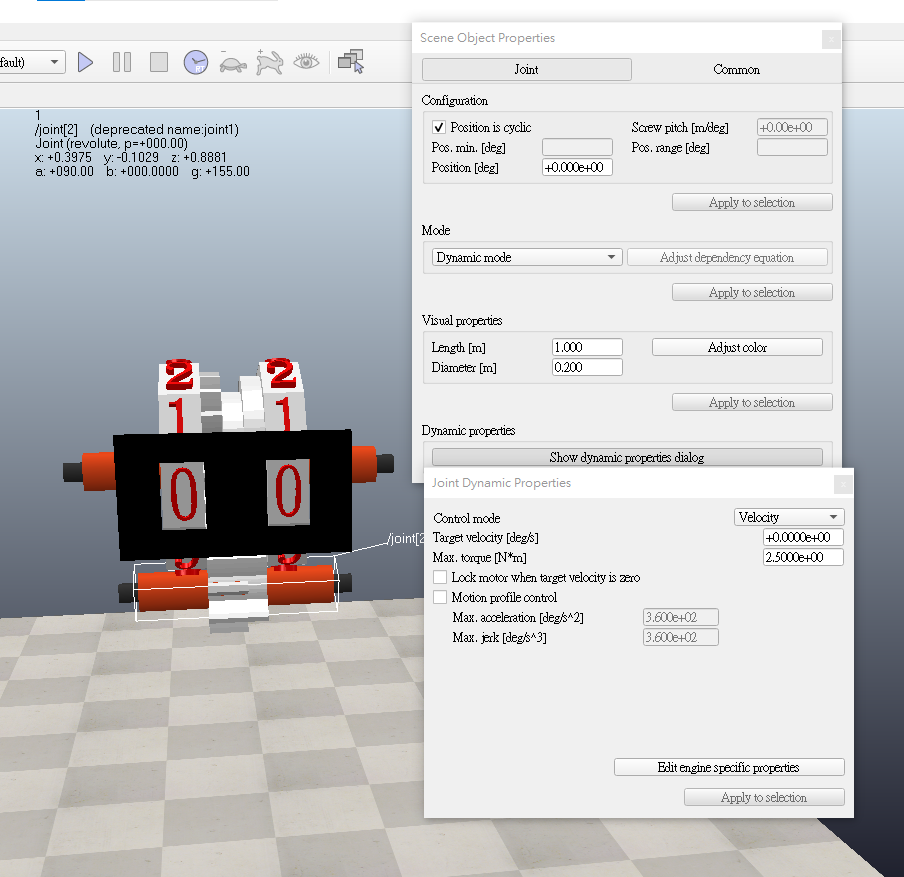
\includegraphics[height=6cm]{28}
\caption{\Large 設定轉速}\label{fig.28}
\end{center}
\end{figure}
\newpage
  調整質量及慣性矩後,記分板即可順利運轉。\\
\begin{figure}[hbt!]
\begin{center}
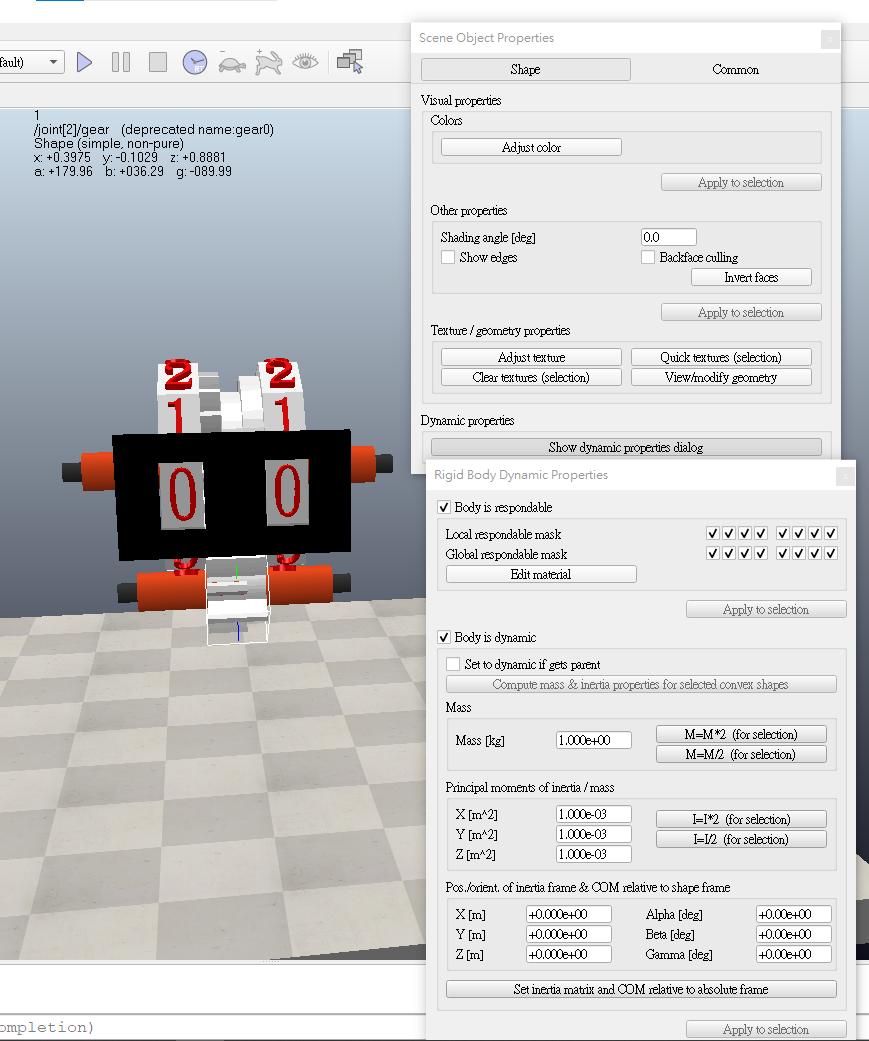
\includegraphics[height=6cm]{29}
\caption{\Large 給定質量}\label{fig.29}
\end{center}
\end{figure}

\newpage
\section{統整場景}
  在球場周圍設置空氣牆,放入 8 名球員,以兩色分為兩隊。\\
\begin{figure}[hbt!]
\begin{center}
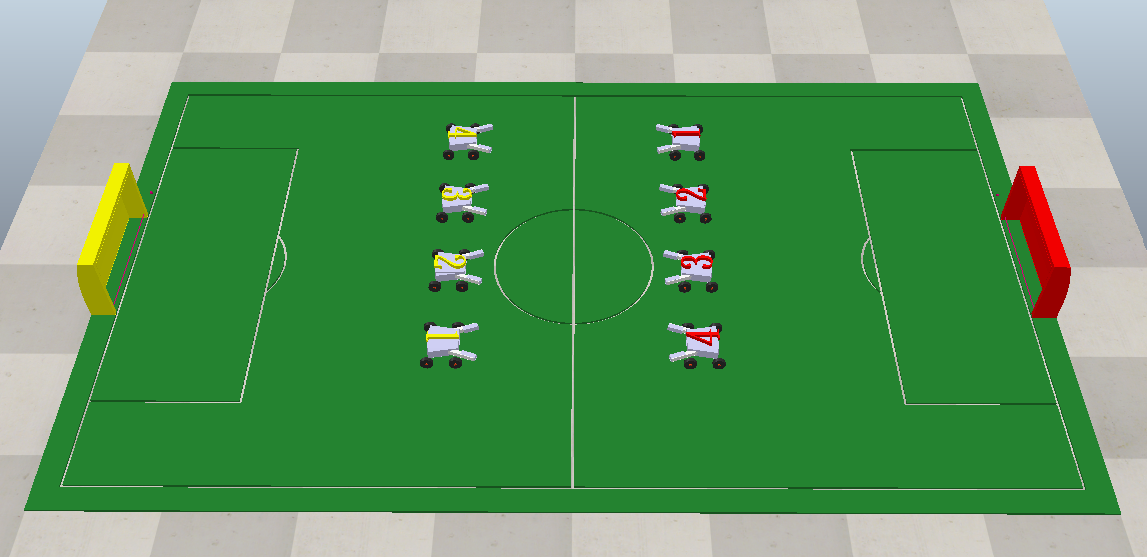
\includegraphics[height=6cm]{60}
\caption{\Large 球場建立}\label{fig.60}
\end{center}
\end{figure}

  以及計時器、LED計分板和機械式記分板。\\
\begin{figure}[hbt!]
\begin{center}
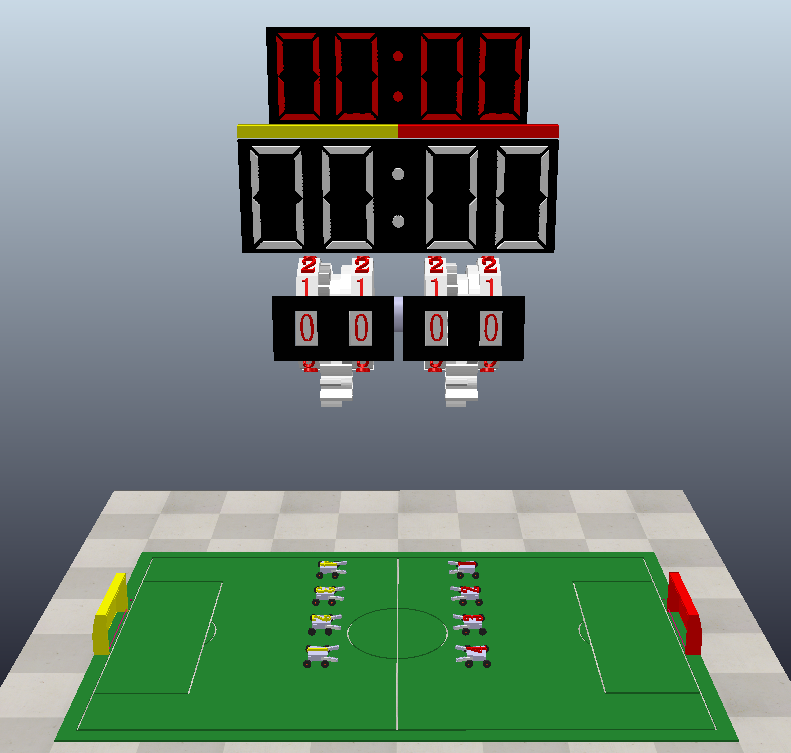
\includegraphics[height=10cm]{61}
\caption{\Large 球場全貌}\label{fig.61}
\end{center}
\end{figure}
\renewcommand{\baselinestretch}{1} %設定行距
\chapter{遠端連線}
\renewcommand{\baselinestretch}{10.0} %設定行距
\pagenumbering{arabic} %設定頁號阿拉伯數字
\setcounter{page}{20}  %設定頁數
\fontsize{14pt}{2.5pt}\sectionef
\section{摘要}
  完成場景建設後,接著要實現跨網路對戰足球機器人。以 zmqRemoteAPI Python 製作控制程式,由組長開起場景,各組員分別跨網路控制各自球員進行賽局,在計時十分鐘的賽局盡可能獲得比對方更高的分數來贏得比賽。\\
\section{連線說明-防火牆}
  從控制台將防火牆都關閉,點開進階設定,組長設定"輸入規則"、組員設定"輸出規則"。新增規則 / 連接埠 / TCP(傳輸控制協定Port) / 特定連接埠 23000-23050,選擇允許連線。\\
\begin{figure}[hbt!]
\begin{center}
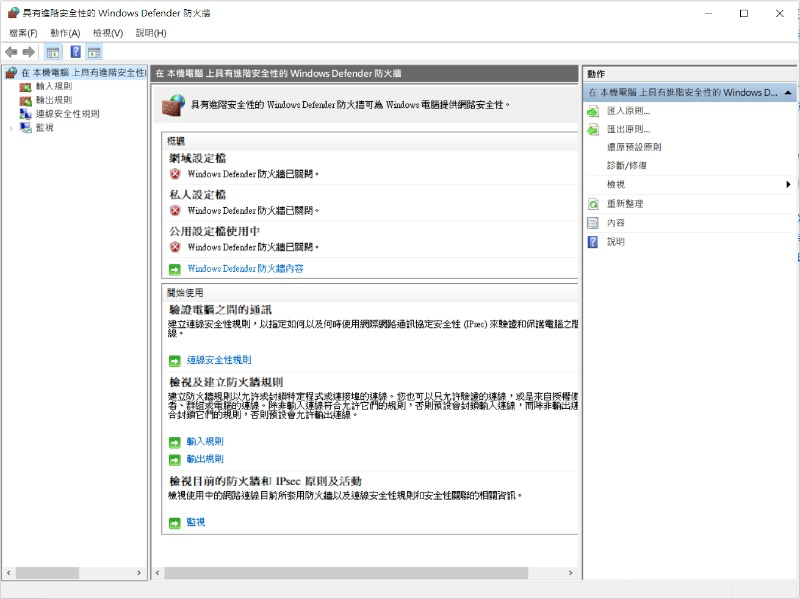
\includegraphics[height=6cm]{03}
\caption{\Large 控制台連接埠}\label{fig.03}
\end{center}
\end{figure}
\section{連線說明-IPv6}
  設定網路 IPv6 位址。\\
\begin{figure}[hbt!]
\begin{center}
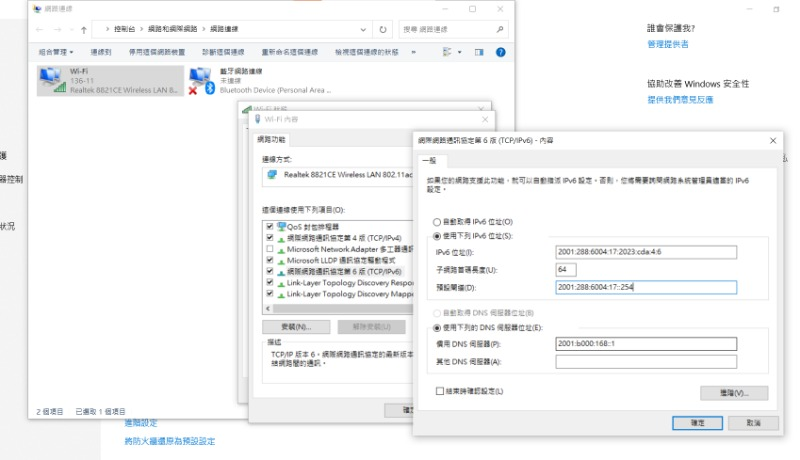
\includegraphics[height=6cm]{07}
\caption{\Large 網路 IPv6 位置}\label{fig.07}
\end{center}
\end{figure}

  下載 CoppeliaSim(4.5.1) 支援 IPv6 版本,zmq 中也需具備 IPv6 環境。\\
\begin{figure}[hbt!]
\begin{center}
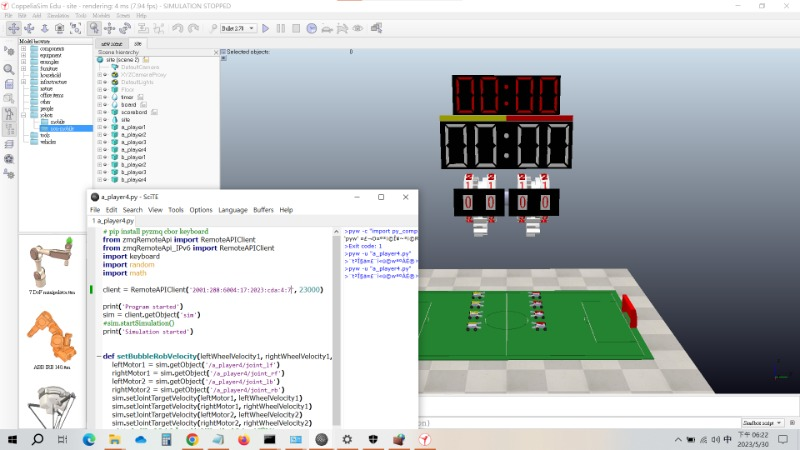
\includegraphics[height=6cm]{08}
\caption{\Large zmq IPv6 }\label{fig.08}
\end{center}
\end{figure}

  接著在 zmq 的 localhost 處打上組長的 IPv6 位置連線。\\
\newpage
\begin{figure}[hbt!]
\begin{center}
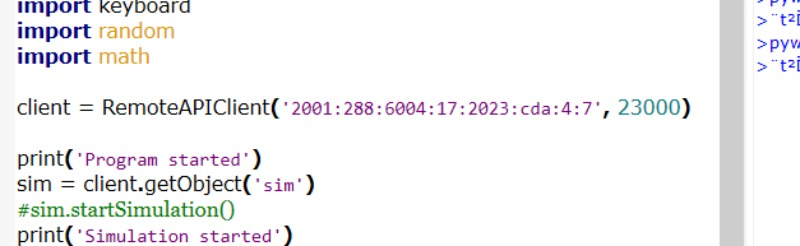
\includegraphics[height=6cm]{09}
\caption{\Large 組長 IPv6 }\label{fig.09}
\end{center}
\end{figure}
  最後在瀏覽器輸入 http://[組長 IP 位置]:23020,即可開啟網頁模擬畫面,完成 pj3 利用多輪車在一足球場景中進行對戰的目標。\\
\renewcommand{\baselinestretch}{1} %設定行距
\chapter{總結}
本學期透過協同合作之方式,從pj1的雙人協同,完成了tutorial1之BubbleRob設計,且在BubbleRob中加上了感測器,載入了lua程式碼,使其擁有避開障礙物之功能。隨後對其加上zmq程式碼使BubbleRob能在CoppeliaSim中由操作者自由移動。接著進入了四人的pj2協同,設計出記分板並加入進球場中,即可進行雙人之足球對戰。再來進行了八人為一組的協同,每位組員分工進行對球場與球員BubbleRob進行改善修正bug,使其對戰更為完善。\\

協同合作可以讓我們對一個項目的開發效率提高,組員可以針對自己的專長與能力來進行任務分配。且協同合作具有共享資源特性,組員之間可以互相學習和激發出創新的想法。隨著科技在不斷的進步,我們為了跟上世界的發展,利用協同合作產品開發的方式是必不可少的。\\
%=---------------------相關資料----------------------=%
%\input{9_reference.tex}
%=---------------附錄-----------------=%
%\addcontentsline{toc}{chapter}{附錄} %新增目錄名稱
%\input{10_appendix.tex}
\newpage
\end{document}
